\documentclass{article}
\usepackage{physics}
\usepackage{graphicx}
\usepackage{caption}
\usepackage{amsmath}
\usepackage{bm}
\usepackage{framed}
\usepackage{authblk}
\usepackage{empheq}
\usepackage{amsfonts}
\usepackage{esint}
\usepackage[makeroom]{cancel}
\usepackage{dsfont}
\usepackage{centernot}
\usepackage{mathtools}
\usepackage{subcaption}
\usepackage{bigints}
\usepackage{amsthm}
\theoremstyle{definition}
\newtheorem{lemma}{Lemma}
\newtheorem{defn}{Definition}[section]
\newtheorem{prop}{Proposition}[section]
\newtheorem{rmk}{Remark}[section]
\newtheorem{thm}{Theorem}[section]
\newtheorem{exmp}{Example}[section]
\newtheorem{prob}{Problem}[section]
\newtheorem{sln}{Solution}[section]
\newtheorem*{prob*}{Problem}
\newtheorem{exer}{Exercise}[section]
\newtheorem*{exer*}{Exercise}
\newtheorem*{sln*}{Solution}
\usepackage{empheq}
\usepackage{tensor}
\usepackage{xcolor}
%\definecolor{colby}{rgb}{0.0, 0.0, 0.5}
\definecolor{MIT}{RGB}{163, 31, 52}
\usepackage[pdftex]{hyperref}
%\hypersetup{colorlinks,urlcolor=colby}
\hypersetup{colorlinks,linkcolor={MIT},citecolor={MIT},urlcolor={MIT}}  
\usepackage[left=1in,right=1in,top=1in,bottom=1in]{geometry}
\setcounter{MaxMatrixCols}{20}
\usepackage{newpxtext,newpxmath}
\newcommand*\widefbox[1]{\fbox{\hspace{2em}#1\hspace{2em}}}

\newcommand{\p}{\partial}
\newcommand{\R}{\mathbb{R}}
\newcommand{\C}{\mathbb{C}}
\newcommand{\lag}{\mathcal{L}}
\newcommand{\nn}{\nonumber}
\newcommand{\ham}{\mathcal{H}}
\newcommand{\M}{\mathcal{M}}
\newcommand{\I}{\mathcal{I}}
\newcommand{\K}{\mathcal{K}}
\newcommand{\F}{\mathcal{F}}
\newcommand{\w}{\omega}
\newcommand{\lam}{\lambda}
\newcommand{\al}{\alpha}
\newcommand{\be}{\beta}
\newcommand{\x}{\xi}

\newcommand{\G}{\mathcal{G}}

\newcommand{\f}[2]{\frac{#1}{#2}}

\newcommand{\ift}{\infty}

\newcommand{\lp}{\left(}
\newcommand{\rp}{\right)}

\newcommand{\lb}{\left[}
\newcommand{\rb}{\right]}

\newcommand{\lc}{\left\{}
\newcommand{\rc}{\right\}}


\newcommand{\V}{\mathbf{V}}
\newcommand{\U}{\mathcal{U}}
\newcommand{\Id}{\mathcal{I}}
\newcommand{\D}{\mathcal{D}}
\newcommand{\Z}{\mathcal{Z}}

%\setcounter{chapter}{-1}


\usepackage{enumitem}



\usepackage{listings}
\captionsetup[lstlisting]{margin=0cm,format=hang,font=small,format=plain,labelfont={bf,up},textfont={it}}
\renewcommand*{\lstlistingname}{Code \textcolor{violet}{\textsl{Mathematica}}}
\definecolor{gris245}{RGB}{245,245,245}
\definecolor{olive}{RGB}{50,140,50}
\definecolor{brun}{RGB}{175,100,80}

%\hypersetup{colorlinks,urlcolor=colby}
\lstset{
	tabsize=4,
	frame=single,
	language=mathematica,
	basicstyle=\scriptsize\ttfamily,
	keywordstyle=\color{black},
	backgroundcolor=\color{gris245},
	commentstyle=\color{gray},
	showstringspaces=false,
	emph={
		r1,
		r2,
		epsilon,epsilon_,
		Newton,Newton_
	},emphstyle={\color{olive}},
	emph={[2]
		L,
		CouleurCourbe,
		PotentielEffectif,
		IdCourbe,
		Courbe
	},emphstyle={[2]\color{blue}},
	emph={[3]r,r_,n,n_},emphstyle={[3]\color{magenta}}
}

\newcommand{\diag}{\text{diag}}
\newcommand{\psirot}{\ket{\psi_\text{rot}(t)} }
\newcommand{\RWA}{\ham_\text{rot}^\text{RWA}}

% 3j symbol
\newcommand{\tj}[6]{ \begin{pmatrix}
		#1 & #2 & #3 \\
		#4 & #5 & #6 
\end{pmatrix}}


\begin{document}
\begin{framed}
\noindent Name: \textbf{Huan Q. Bui}\\
Course: \textbf{8.421 - AMO I}\\
Problem set: \textbf{\#8}\\
Due: Friday, April 8, 2022.
\end{framed}
	

\noindent \textbf{1. Optical Traps and Scattering.} What are are the proper power and wavelength needed to trap an ultracold atomic gas? Consider an alkali atom with resonance frequency $\omega_0$ on the principal $nS \to nP$ transition. A sample of atoms in the ground state $nS$ are exposed to monochromatic radiation of intensity $I$ and frequency $\omega_L < \omega_0$.  Using the fact that essentially all of the oscillator strength out of the ground state comes from the $nS \to nP$ transition, we have
\begin{align*}
\alpha(\omega_L) \approx \f{2e^2}{\hbar} \abs{\bra{nP} z \ket{nS}}^2 \f{\omega_0}{\omega_0^2 - \omega_L^2} \implies \abs{\bra{nP} z \ket{nS}}^2 = \f{\hbar \al(\omega_L)}{2e^2} \f{\omega_0^2 - \omega_L^2}{\omega_0}.
\end{align*} 

\begin{enumerate}[label=(\alph*)]
	\item AC Stark shift: 
	
	\begin{enumerate}[label=(\roman*)]
		\item From lecture, the AC Stark shift $U_i$ from time-dependent perturbation theory is given by 
		\begin{align*}
		U_i = -\f{1}{4}\al(\omega_L) \mathcal{E}^2 = -\f{2I\al(\omega_L)}{4c\epsilon_0} = -\f{I\al(\omega_L)}{2c\epsilon_0}.
		\end{align*}
		
		
		\item Now, we want to use the rotating wave approximation to obtain the AC Stark shift. This can be done by first writing down the true (symmetrized) Hamiltonian:
		\begin{align*}
		\ham = \f{\hbar}{2}\begin{pmatrix}
		-\omega_0 & \omega_R e^{i\omega_L t} \\ \omega_R^* e^{-i\omega_L t} & \omega_0
		\end{pmatrix}.
		\end{align*}
		By going into the rotating frame, plus making the rotating wave approximation, we find that
		\begin{align*}
		\ham_\text{rot}^\text{RWA} = \f{\hbar}{2}\begin{pmatrix}
		-\delta & \omega_R \\ \omega_R & \delta
		\end{pmatrix}
		\end{align*}
		where $\delta = \omega_0 - \omega_L$. The energy shifts can be obtained from the eigenvalues:
		\begin{align*}
		\Delta E = \pm  \f{\hbar}{2}\sqrt{\omega_R^2 + \delta^2} =\pm \f{\hbar}{2}\sqrt{\omega_R^2 + (\omega_0 - \omega_L)^2} \approx \pm \f{\hbar(\omega_0 - \omega_L)}{2} \pm \f{\hbar \omega_R^2}{4(\omega_0 - \omega_L)}
		\end{align*}
		where we have used the fact that $\omega_R \ll \abs{\omega_0 - \omega_L}$. From here, we find that the shift is 
		\begin{align*}
		U_{ii} = -\f{\hbar \omega_R^2}{4(\omega_0 - \omega_L)} 
		\end{align*}
		In particular, the energy of the lower state gets shifted down while the energy of the higher state gets shifted up (since we're red-detuning). 
		
		
		\item From the previous two parts, we find that
		\begin{align*}
		\f{U_i}{U_{ii}} = \f{I\al(\omega_L)}{2c\epsilon_0} \f{4(\omega_0 - \omega_L)}{\hbar \omega_R^2}  = \f{I}{c\epsilon_0 \omega_R^2 }\f{4e^2}{\hbar^2} \abs{\bra{nP} z \ket{nS}}^2 \f{\omega_0}{\omega_0 + \omega_L}.
		\end{align*}
		To simplify this, we must write the Rabi frequency in terms of the intensity:
		\begin{align*}
			\omega_R = \f{e\mathcal{E}|\bra{nS} z \ket{nP}|}{\hbar} \implies \omega_R^2 = \f{e^2|\bra{nS} z \ket{nP}|^2}{\hbar^2} \f{2I}{c\epsilon_0}.
		\end{align*}
		With this, we have
		\begin{align*}
			{\f{U_{i}}{U_{ii}} = \f{2\omega_0}{\omega_0 + \omega_L}}
		\end{align*}
		When $\omega_L \approx 0$, we have
		\begin{align*}
		\f{U_i}{U_{ii}} \approx 2.
		\end{align*}
		When $\omega_L \approx \omega_0$, we may write $\omega_L + \omega_0 = 2\omega_0$, so that
		\begin{align*}
		\f{U_i}{U_{ii}} \approx 1.
		\end{align*}
	\end{enumerate}
	We see that if the intensity has spatial structure, with the appropriate detuning, the AC Stark shift can have energy minima where the atoms can be trapped. 
	
	\item From time-dependent perturbation theory, the amplitude of the excited state is
	\begin{align*}
	c_2(t) =  \f{e\mathcal{E}}{2\hbar} \bra{nS} z \ket{nP} \lb \f{e^{i(\omega_0+\omega_L)t}-1}{\omega_0-\omega_L} + \f{e^{i(\omega_0-\omega_L)t}-1}{\omega_0+\omega_L} \rb.
	\end{align*}
	Ignoring the $-1$ terms which are associated with transients, we have
	\begin{align*}
		P_e(t) = \f{e^2\mathcal{E}^2}{4\hbar^2}|\bra{nS}z \ket{nP}|^2 \f{2[\omega_0^2+\omega_L^2+(\omega_0^2-\omega_L^2)\cos(2\omega_L t)]}{(\omega_0^2-\omega_L^2)^2}.
	\end{align*}
	After time-averaging, this quantity is 
	\begin{align*}
		P_{e,i} = {\f{\omega_R^2}{2} \f{\omega_0^2+\omega_L^2}{(\omega_0^2-\omega_L^2)^2}}
	\end{align*}


	In the RWA picture, we know that
	\begin{align*}
	P_{e,ii}(t) = \f{\omega_R^2}{\omega^2_R + \delta^2} \sin^2 \lp \f{\sqrt{\omega_R^2 + (\omega_0 - \omega_L)^2} t}{2} \rp.
	\end{align*}
	After time-averaging this is 
	\begin{align*}
	P_{e,ii} = \f{\omega_R^2}{2(\omega^2_R + \delta^2)} \approx  {\f{\omega_R^2}{2 (\omega_0 - \omega_L)^2}}
	\end{align*}
	where we have used the approximation that the Rabi frequency is much less than the detuning.
	
	\item Calculate the photon scattering rate:
	
	\begin{enumerate}[label=(\roman*)]
		\item Starting with
		\begin{align*}
			P = \f{ck^4|\bm{d}|^2}{3} = \f{\omega_L^4}{3c^3}\abs{\bm{d}}^2,
		\end{align*}
		if we say $d = \al(\omega_L)\mathcal{E}$ then we have
		\begin{align*}
			R_\text{sc} &= \f{P}{\hbar \omega_L}= \f{\omega_L^3}{3\hbar c^3}\abs{\al(\omega_L)}^2 \mathcal{E}^2= \f{\omega_L^3}{3\hbar c^3}\abs{\al(\omega_L)}^2 \f{8\pi I}{c}
		\end{align*}
		where we have converted the intensity into CGS units. Now we recall from perturbation theory that
		\begin{align*}
			\al(\omega_L) = \f{2e^2}{\hbar} |\bra{nS} z \ket{nP}|^2 \f{\omega_0}{\omega_0^2 - \omega_L^2} = \f{e^2}{\hbar} |\bra{nS} z \ket{nP}|^2 \lp \f{1}{\omega_0 - \omega_L} + \f{1}{\omega_0 + \omega_L} \rp.
		\end{align*}
		From here we find that
		\begin{align*}
			|\al(\omega_L)|^2 = \f{e^4}{\hbar^2} |\bra{nS} z \ket{nP}|^4 \lp \f{1}{\omega_0 - \omega_L} + \f{1}{\omega_0 + \omega_L} \rp^2.
		\end{align*}
		Putting everything together, we find 
		\begin{align*}
			R_\text{sc,i} &= \f{\omega_L^3}{3\hbar c^3}\f{8\pi I}{c}\f{e^4}{\hbar^2} |\bra{nS} z \ket{nP}|^4 \lp \f{1}{\omega_0 - \omega_L} + \f{1}{\omega_0 + \omega_L} \rp^2\\
			&= \f{8\pi I\omega_L^3 e^4}{3 c^4 \hbar^3} |\bra{nS} z \ket{nP}|^4 \lp \f{1}{\omega_0 - \omega_L} + \f{1}{\omega_0 + \omega_L} \rp^2.
		\end{align*}
		Under RWA, we simply drop the counter-rotating term to find 
		\begin{align*}
			R_\text{sc,ii}= \f{8\pi I\omega_L^3 e^4}{3 c^4 \hbar^3} |\bra{nS} z \ket{nP}|^4 \lp \f{1}{\omega_0 - \omega_L} \rp^2.
		\end{align*}
		
		\item Let us write $R_\text{cs,i}$ and $R_\text{sc,ii}$ in terms of the spontaneous emission rate $\Gamma = 4e^2 \omega_0^3 |\bra{nS}z\ket{nP}|^2/3\hbar c^3$: 
		\begin{align*}
			R_\text{sc,i} &= \f{8\pi I\omega_L^3 e^4}{3 c^4 \hbar^3} |\bra{nS} z \ket{nP}|^4 \lp \f{1}{\omega_0 - \omega_L} + \f{1}{\omega_0 + \omega_L} \rp^2 \\
			&= \f{8\pi I\omega_L^3 }{3 c^4 \hbar^3} \f{9\Gamma^2 \hbar^2 c^6}{16\omega_0^6}  \lp \f{1}{\omega_0 - \omega_L} + \f{1}{\omega_0 + \omega_L} \rp^2\\
			&= \f{3\pi c^2}{2\hbar \omega_0^3}\lp \f{\omega_L}{\omega_0} \rp^3 \lp \f{\Gamma}{\omega_0 - \omega_L} + \f{\Gamma}{\omega_0 + \omega_L} \rp^2 I,
		\end{align*}
	which is a standard result. Making the RWA, we find
	\begin{align*}
		R_\text{sc,ii} &= \f{3\pi c^2}{2\hbar \omega_0^3}\lp \f{\omega_L}{\omega_0} \rp^3 \lp \f{\Gamma}{\omega_0 - \omega_L}  \rp^2 I.
	\end{align*}
	From Part (b), we have that
	\begin{align*}
		P_{e,ii} &= \f{\omega_R^2}{2(\omega_0 - \omega_L)^2},
	\end{align*}
	which gives
	\begin{align*}
		R_\text{sc,ii} &=  \f{3\pi c^2}{2\hbar \omega_0^3}\lp \f{\omega_L}{\omega_0} \rp^3 \lp \f{\Gamma}{\omega_0 - \omega_L}  \rp^2 I \\
		&= \f{3\pi c^2}{2\hbar \omega_0^3}\lp \f{\omega_L}{\omega_0} \rp^3 \f{I\Gamma^2 }{\omega_R^2} 2P_{e,ii}\\
		&= \f{3\pi c^2}{\hbar \omega_0^3}\lp \f{\omega_L}{\omega_0} \rp^3 \Gamma^2 P_{e,ii} \f{\hbar^2}{e^2}\f{c}{8\pi} \f{4e^2\omega_0^3}{3\hbar c^3 \Gamma}\\
		&= \boxed{\f{ 1}{2}\lp \f{\omega_L}{\omega_0} \rp^3 \Gamma P_{e,ii}}
	\end{align*}
	
	
	
	
		\item (Optional) We describe scattering as spontaneous emission from a virtual energy level. Figure \ref{fig:1} shows the energy diagram for this description. We may identify the photon scattering rate as the decay rate from this virtual state. The lifetime of this virtual state is then found by inverting $R_\text{sc}$: 
		\begin{align*}
		\tau_\text{virtual} = \f{1}{R_\text{sc,i}} = 
		\f{2\hbar \omega_0^3}{ 3\pi c^2 I  }
		\lp \f{\omega_0}{\omega_L} \rp^3 \lp \f{\Gamma}{\omega_0 - \omega_L} + \f{\Gamma}{\omega_0 + \omega_L} \rp^{-2} 
		\end{align*}
		
		
		\begin{figure}[!htb]
			\centering
			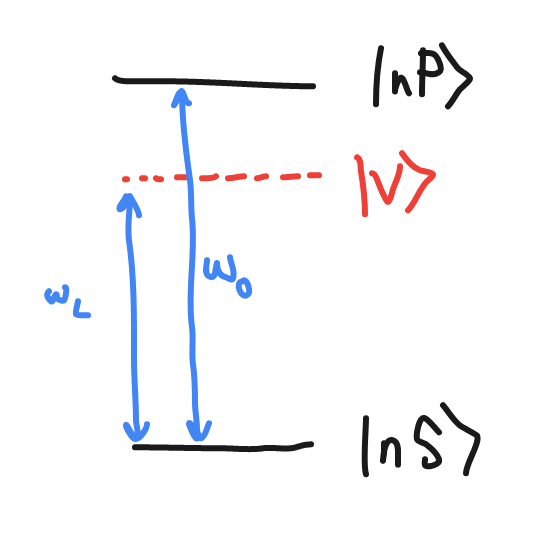
\includegraphics[width=0.35\textwidth]{virtual.png}
			\caption{we may describe scattering as spontaneous emission from a virtual energy level.}
			\label{fig:1}
		\end{figure}
		
		
		
	\end{enumerate}
	
	\item 
	
	\begin{enumerate}[label=(\roman*)]
		\item  The $D_{1,2}$ lines of Na have $\omega_0 \approx 2\pi \cdot 508 $ THz. Now the infrared laser at 985 nm has $\omega_L = 2\pi \cdot 304$ THz, which corresponds to a detuning of $2\pi\cdot 204$ THz, which is much larger than the detuning of the yellow laser (a few GHz). This means that the RWA expression is more suitable for the yellow laser. 
		
		\item Here we want to calculate the required power and scattering rate for each of the two types of lasers. Using results from time-dependent perturbation theory, we have two equations:
		\begin{align*}
			&U_i = \f{I(0) \al(\omega_L)}{2c\epsilon_0} =   \f{3\pi c^2}{2\omega_0^3} \lp \f{\Gamma}{\omega_0 - \omega_L} + \f{\Gamma}{\omega_0 + \omega_L}\rp I(0) = k_B \cdot 10 \, \mu\text{K} \\
			& R_\text{sc,i} = \f{3\pi c^2}{2\hbar \omega_0^3}\lp \f{\omega_L}{\omega_0} \rp^3 \lp \f{\Gamma}{\omega_0 - \omega_L} + \f{\Gamma}{\omega_0 + \omega_L} \rp^2 I(0).
		\end{align*}
	where we have converted to CGS units in the first line. To solve for $P,R_{\text{sc,ii}}$, we will use $I(0)=2P/\pi w^2$ and Mathematica. For each laser, we will have:
	\begin{align*}
		\text{Yellow laser: } \,\,& 
		P = 0.102 \,\mu\text{W}; \quad 
		R_{\text{sc,ii}} = 7700 \,\text{Hz}\\
		\text{Infrared laser:}\,\,&  
		P = 9.871 \, \text{mW}; \quad 
		R_{\text{sc,ii}} = 0.017 \,\text{Hz}
	\end{align*}

	Mathematica calculations:
	\begin{lstlisting}
		In[1]:= Solve[(2*P/(Pi*w^2))*3*Pi*c^2*
		Gam*(1/(omega0 - omegaL) + 1/(omega0 + omegaL))/(2*omega0^3) == 
		kB*T, P]
		
		Out[1]= {{P -> (
				kB omega0^2 (omega0 - omegaL) (omega0 + omegaL) T w^2)/(6 c^2 Gam)}}
		
		In[15]:= numbers = {kB -> 1.3806*10^(-23),
			omega0 -> 2*Pi*3*10^8/(589*10^-9),
			omegaL -> 2*Pi*3*10^8/(985*10^-9),
			T -> 10*10^(-6),
			w -> 6*10^(-6),
			Gam -> 2*Pi*10*10^6,
			c -> 3*10^8,
			hbar -> 1.0545*10^(-34)};
		
		In[16]:= (kB omega0^2 (omega0 - omegaL) (omega0 + omegaL) T w^2)/(
		6 c^2 Gam) /. numbers
		
		Out[16]= 0.00987114
		
		In[17]:= R = ((3*Pi*c^2)/(2*hbar*omega0^3))*(omegaL/
		omega0)^3*(Gam/(omega0 - omegaL) + Gam/(omega0 + omegaL))^2*2*
		P/(Pi*w^2);
		
		In[18]:= R /. numbers /. {P -> 0.009871144461932576`}
		
		Out[18]= 0.0171102
	\end{lstlisting}
	\end{enumerate}
\end{enumerate}


\noindent \textbf{2. Magic Wavelength Optical Trap.} Here we have a system with lower state $\ket{S}$, upper state $\ket{P}$ with bare energy separation $\hbar \omega_{PS}$. The dipole moment is $d_{PS}$. 

\begin{enumerate}[label=(\alph*)]
	\item 
	
	\begin{enumerate}[label=(\roman*)]
		\item The AC Stark shift for the state $S$ is given by 
		\begin{align*}
			\Delta E_S = -\f{1}{4}\al(\omega_L) \mathcal{E}^2 = -\f{d_{PS}^2\mathcal{E}^2}{4\hbar}\lp \f{1}{\omega_{PS} - \omega_L} + \f{1}{\omega_{PS} + \omega_L} \rp
		\end{align*}
		Nothing too surprising here.
		
		\item Assuming that state $\ket{P}$ couples almost exclusively to state $\ket{S}$ only, then the polarizability of state $\ket{P}$ is simply the additive reciprocal of the polarizability of state $\ket{S}$. This means that the energy shift of state $\ket{P}$ is 
		\begin{align*}
		\Delta E_S = -\Delta E_P.
		\end{align*}
		
		\item Since the energy levels shift either \textit{away from} or \textit{toward} each other as a function of the detuning, it is not possible for the relative energy shift to be zero with the current setup. For that to happen, we will need a third level.
	\end{enumerate}
	
	\item Consider a third, higher energy state $\ket{D}$ and assume that the states $\ket{S}$ and $\ket{D}$ do not couple directly. With this information, we know that the energy shift in $\ket{S}$ remains the same. 
	
	\begin{enumerate}[label=(\roman*)]
		\item Since $\ket{P}$ couples with $\ket{D}$, the energy shift is modified. 
		\begin{align*}
		\Delta E_P &= -\Delta E_S -\f{d_{PD}^2 \mathcal{E}^2}{4\hbar}\lp \f{1}{\omega_{DP} - \omega_L} + \f{1}{\omega_{DP} + \omega_L} \rp\\
		&= \f{d_{PS}^2\mathcal{E}^2}{4\hbar}\lp \f{1}{\omega_{PS} - \omega_L} + \f{1}{\omega_{PS} + \omega_L} \rp -\f{d_{PD}^2 \mathcal{E}^2}{4\hbar}\lp \f{1}{\omega_{DP} - \omega_L} + \f{1}{\omega_{DP} + \omega_L} \rp\\
		&= \f{n^2d_{DP}^2\mathcal{E}^2}{4\hbar}\lp \f{1}{f\omega_{DP} - \omega_L} + \f{1}{f\omega_{DP} + \omega_L} \rp -\f{d_{PD}^2 \mathcal{E}^2}{4\hbar}\lp \f{1}{\omega_{DP} - \omega_L} + \f{1}{\omega_{DP} + \omega_L} \rp
		\end{align*}
		
		\item We would like to set the $\ket{S}\to \ket{P}$ transition frequency so that it is independent of the trap laser power. This is achieved exactly when the shifts in $\ket{S}$ and in $\ket{P}$ are the same:
		\begin{align*}
		&2\f{n^2d_{DP}^2\mathcal{E}^2}{4\hbar}\lp \f{1}{f\omega_{DP} - \omega_L} + \f{1}{f\omega_{DP} + \omega_L} \rp = \f{d_{PD}^2 \mathcal{E}^2}{4\hbar}\lp \f{1}{\omega_{DP} - \omega_L} + \f{1}{\omega_{DP} + \omega_L} \rp\\
		&\iff \boxed{\omega_L = \omega_{DP} \sqrt{\f{f(f-2n^2)}{1-2fn^2}}  }
		\end{align*}
		
		
	\end{enumerate}
\end{enumerate}


\noindent \textbf{3. Species-Dependent and Spin-Dependent AC Stark shift}	
	
\begin{enumerate}[label=(\alph*)]
	\item Here we consider a linearly polarized dipole trap laser with electric field polarization along the $x$ direction propagating along the $z$ direction. 
	
	\begin{enumerate}[label=(\roman*)]
		\item For this part we want to find the laser wavelength for which the AC Stark shift in state $\ket{S}_{1/2}$ is zero. The AC Stark shift is given by 
		\begin{align*}
			\Delta E_S = -\f{\mathcal{E}^2}{4\hbar} \sum_i \abs{C_{1,i}}^2 \lb \f{1}{\omega_1 - \omega} + \f{1}{\omega_1+\omega} \rb  -\f{\mathcal{E}^2}{4\hbar} \sum_i |C_{2,i}|^2 \lb \f{1}{\omega_2 - \omega} + \f{1}{\omega_2+\omega} \rb
		\end{align*}
	where $C_{1,i}, C_{2,i}$ are the dipole matrix elements. We can calculate the sums:
	\begin{align*}
		 \sum_i \abs{C_{1,i}}^2 &= \f{1}{2}\abs{e\bra{S_{1/2},+1/2} \hat{\sigma}_-\cdot \bm{r} \ket{P_{1/2},-1/2}}^2 + \f{1}{2} \abs{e\bra{S_{1/2},-1/2} \hat{\sigma}_-\cdot \bm{r}   \ket{P_{1/2},+1/2}}^2 = \f{2d_1^2}{3}\\
		 \sum_i \abs{C_{2,i}}^2 &= \f{1}{2}\abs{e\bra{S_{1/2},+1/2} \hat{\sigma}_+\cdot \bm{r} \ket{P_{3/2},+3/2}}^2 + \f{1}{2} \abs{e\bra{S_{1/2},+1/2} \hat{\sigma}_-\cdot \bm{r}   \ket{P_{3/2},-1/2}}^2\\
		 & + \f{1}{2}\abs{e\bra{S_{1/2},-1/2} \hat{\sigma}_+\cdot \bm{r} \ket{P_{3/2},+1/2}}^2 + \f{1}{2} \abs{e\bra{S_{1/2},-1/2} \hat{\sigma}_-\cdot \bm{r}   \ket{P_{3/2},-3/2}}^2 = \f{4d_2^2}{3}
	\end{align*}
	where we have used
	\begin{align*}
		\bra{a} \hat{x} \cdot \bm{r} \ket{b} = \f{1}{\sqrt{2}}  \bra{a} \hat{\sigma}_+ \cdot \bm{r} \ket{b} + \f{1}{\sqrt{2}} \bra{a} \hat{\sigma}_- \cdot \bm{r} \ket{b}
	\end{align*}
	and fact that the inference terms between the different polarizations vanish for this problem. From here, we find 
	\begin{align*}
	\Delta E_S = -\f{\mathcal{E}^2}{4\hbar}\lb \f{2d_1^2}{3}\lp \f{1}{\omega_1-\omega} + \f{1}{\omega_1+\omega} \rp + \f{4d_2^2}{3}\lp \f{1}{\omega_2-\omega} + \f{1}{\omega_2+\omega} \rp \rb.
	\end{align*}
	This quantity vanishes exactly when 
	\begin{align*}
	\omega = \sqrt{\f{\omega_1\omega_2( d_1^2\omega_2 + 2d_2^2\omega_1)}{d_1^2 \omega_1 + 2d_2^2\omega_2 }}.
	\end{align*}
	With $\lambda_1 = 795$ nm, $\lambda_2 = 780$ nm, $d_1 = 3 ea_0$, $d_2 = 4.2 ea_0$, we find 
	\begin{align*}
	\boxed{\lambda \approx 792 \text{ nm}}
	\end{align*}
	
	
	Calculation in Mathematica:
	\begin{lstlisting}
	In[3]:= Solve[
	2 d1^2/3*(1/(o1 - o) + 1/(o1 + o)) + 
	4 d2^2/3*(1/(o2 - o) + 1/(o2 + o)) == 0, o] // FullSimplify
	
	Out[3]= {{o -> -(Sqrt[o1 o2 (2 d2^2 o1 + d1^2 o2)]/Sqrt[
	d1^2 o1 + 2 d2^2 o2])}, {o -> Sqrt[o1 o2 (2 d2^2 o1 + d1^2 o2)]/
	Sqrt[d1^2 o1 + 2 d2^2 o2]}}
	
	In[5]:= Lam = 
	2*Pi*c/(Sqrt[o1 o2 (2 d2^2 o1 + d1^2 o2)]/Sqrt[d1^2 o1 + 2 d2^2 o2]);
	
	In[10]:= subs = {o1 -> 2*Pi*3*10^8/(795*10^-9),
	o2 -> 2*Pi*3*10^8/(780*10^-9),
	d1 -> 3*(1.602*10^-19)*0.529*10^-10,
	d2 -> 4.2*(1.602*10^-19)*0.529*10^-10,
	c -> 3*10^8};
	
	In[11]:= Lam /. subs
	
	Out[11]= 7.91928*10^-7
	\end{lstlisting}
		
		
		\item The wavelength we find above is near the experimentally determined wavelength of 789.85(1) nm, but not quite. The discrepancy of $\sim$ 6 THz is due to the fact that we are neglecting hyperfine structure of the ground state. Theoretical predictions for $\lambda$ that include hyperfine structure are accurate to about $0.04$ nm.  See Table II of  L. J. LeBlanc and J. H. Thywissen, \textit{Phys. Rev. A} \textbf{75},
		053612 (2007).
		

	\end{enumerate}
	
	\item For this part we consider $\sigma_+$ polarized light that is much closer to the $S_{1/2}\to P_{3/2}$ transition and ignore coupling to the $P_{1/2}$ state. 
	
	\begin{enumerate}[label=(\roman*)]
		\item Here we calculate the AC Stark shift for the two states $\ket{S_{1/2},+1/2}$ and $\ket{S_{1/2}, -1/2}$:
		\begin{align*}
		\Delta E_{\ket{S_{1/2},+1/2}} 
		&= -\f{\mathcal{E}^2}{4\hbar} \abs{ e\bra{S_{1/2},+1/2} \hat{\sigma}_+ \cdot \bm{r} \ket{P_{3/2},+3/2}}^2  \lp\f{1}{\omega_2 - \omega} + \f{1}{\omega_2 + \omega} \rp\\
		&= -\f{\mathcal{E}^2d_2^2}{4\hbar} \lp\f{1}{\omega_2 - \omega} + \f{1}{\omega_2 + \omega} \rp.
		\end{align*}
		\begin{align*}
		\Delta E_{\ket{S_{1/2},-1/2}} &= -\f{\mathcal{E}^2}{4\hbar}  \abs{ e\bra{S_{1/2},-1/2} \hat{\sigma}_+ \cdot \bm{r} \ket{P_{3/2},+1/2}}^2  \lp\f{1}{\omega_2 - \omega} + \f{1}{\omega_2 + \omega} \rp\\
		&\,\,\,+
		-\f{\mathcal{E}^2}{4\hbar}\abs{ e\bra{S_{1/2},-1/2} \hat{\sigma}_+ \cdot \bm{r} \ket{P_{1/2},+1/2}}^2  \lp\f{1}{\omega_1 - \omega} + \f{1}{\omega_1 + \omega} \rp\\
		&=  -\f{\mathcal{E}^2}{4\hbar} \lb \f{d_2^2}{3}  \lp\f{1}{\omega_2 - \omega} + \f{1}{\omega_2 + \omega} \rp  + \f{2d_1^2}{3} \lp\f{1}{\omega_1 - \omega} + \f{1}{\omega_1 + \omega} \rp \rb.
		\end{align*}
		
		
		
		\item Let us attempt to make a general expression for the AC Stark shift which gives us the two answers above depending on which $m_J$ we use. Let us write the AC Stark shift as 
		\begin{align*}
		U = U_S + U_V = U_S + g_J m_J \mu_B B_\text{eff} = U_S + 2 m_J \mu_B B_\text{eff}.
		\end{align*}
		For $m_J = -1/2$ we have
		\begin{align*}
		U_S - \mu_B B_\text{eff} = -\f{\mathcal{E}^2d_2^2}{4\hbar} \lp\f{1}{\omega_2 - \omega} + \f{1}{\omega_2 + \omega} \rp.
		\end{align*}
		For $m_J = 1/2$ we have
		\begin{align*}
		U_S + \mu_B B_\text{eff} = -\f{\mathcal{E}^2}{4\hbar} \lb \f{d_2^2}{3}  \lp\f{1}{\omega_2 - \omega} + \f{1}{\omega_2 + \omega} \rp  + \f{2d_1^2}{3} \lp\f{1}{\omega_1 - \omega} + \f{1}{\omega_1 + \omega} \rp \rb.
		\end{align*}
		Solving for $U_S$ and $B_\text{eff}$ we find 
		\begin{align*}
		U_S = -\f{\mathcal{E}^2}{8\hbar} \lb \f{4d_2^2}{3}  \lp\f{1}{\omega_2 - \omega} + \f{1}{\omega_2 + \omega} \rp  + \f{2d_1^2}{3} \lp\f{1}{\omega_1 - \omega} + \f{1}{\omega_1 + \omega} \rp \rb
		\end{align*}
		and 
		\begin{align*}
		B_\text{eff} = -\f{\mathcal{E}^2}{8\mu_B\hbar} \lb -\f{2d_2^2}{3}  \lp\f{1}{\omega_2 - \omega} + \f{1}{\omega_2 + \omega} \rp  + \f{2d_1^2}{3} \lp\f{1}{\omega_1 - \omega} + \f{1}{\omega_1 + \omega} \rp \rb.
		\end{align*}
		This fictitious magnetic field points along the quantization axis. 
		
		
	\end{enumerate}
\end{enumerate}
	
	
\end{document}








